%\documentclass[a4paper]{fhnwreport} %Legt grundlegende Formatierungen wie Schriftarten, Ort Seitenzahlen etc. fest.
%
%\graphicspath{{./graphics/}}%Change according to graphics folder!
%
%\begin{document}

\section{Hardware}

Der Sensorprint wird über das Solarpanel gespiesen. Es ist deshalb darauf zu achten, das die Leistung nicht mehr als 100mW beträgt.

Die Kommunikation über die Powerline (PLC) wird mittels eines Powerline Transceivers/Receivers realisiert.
\begin{figure}[h]
\centering
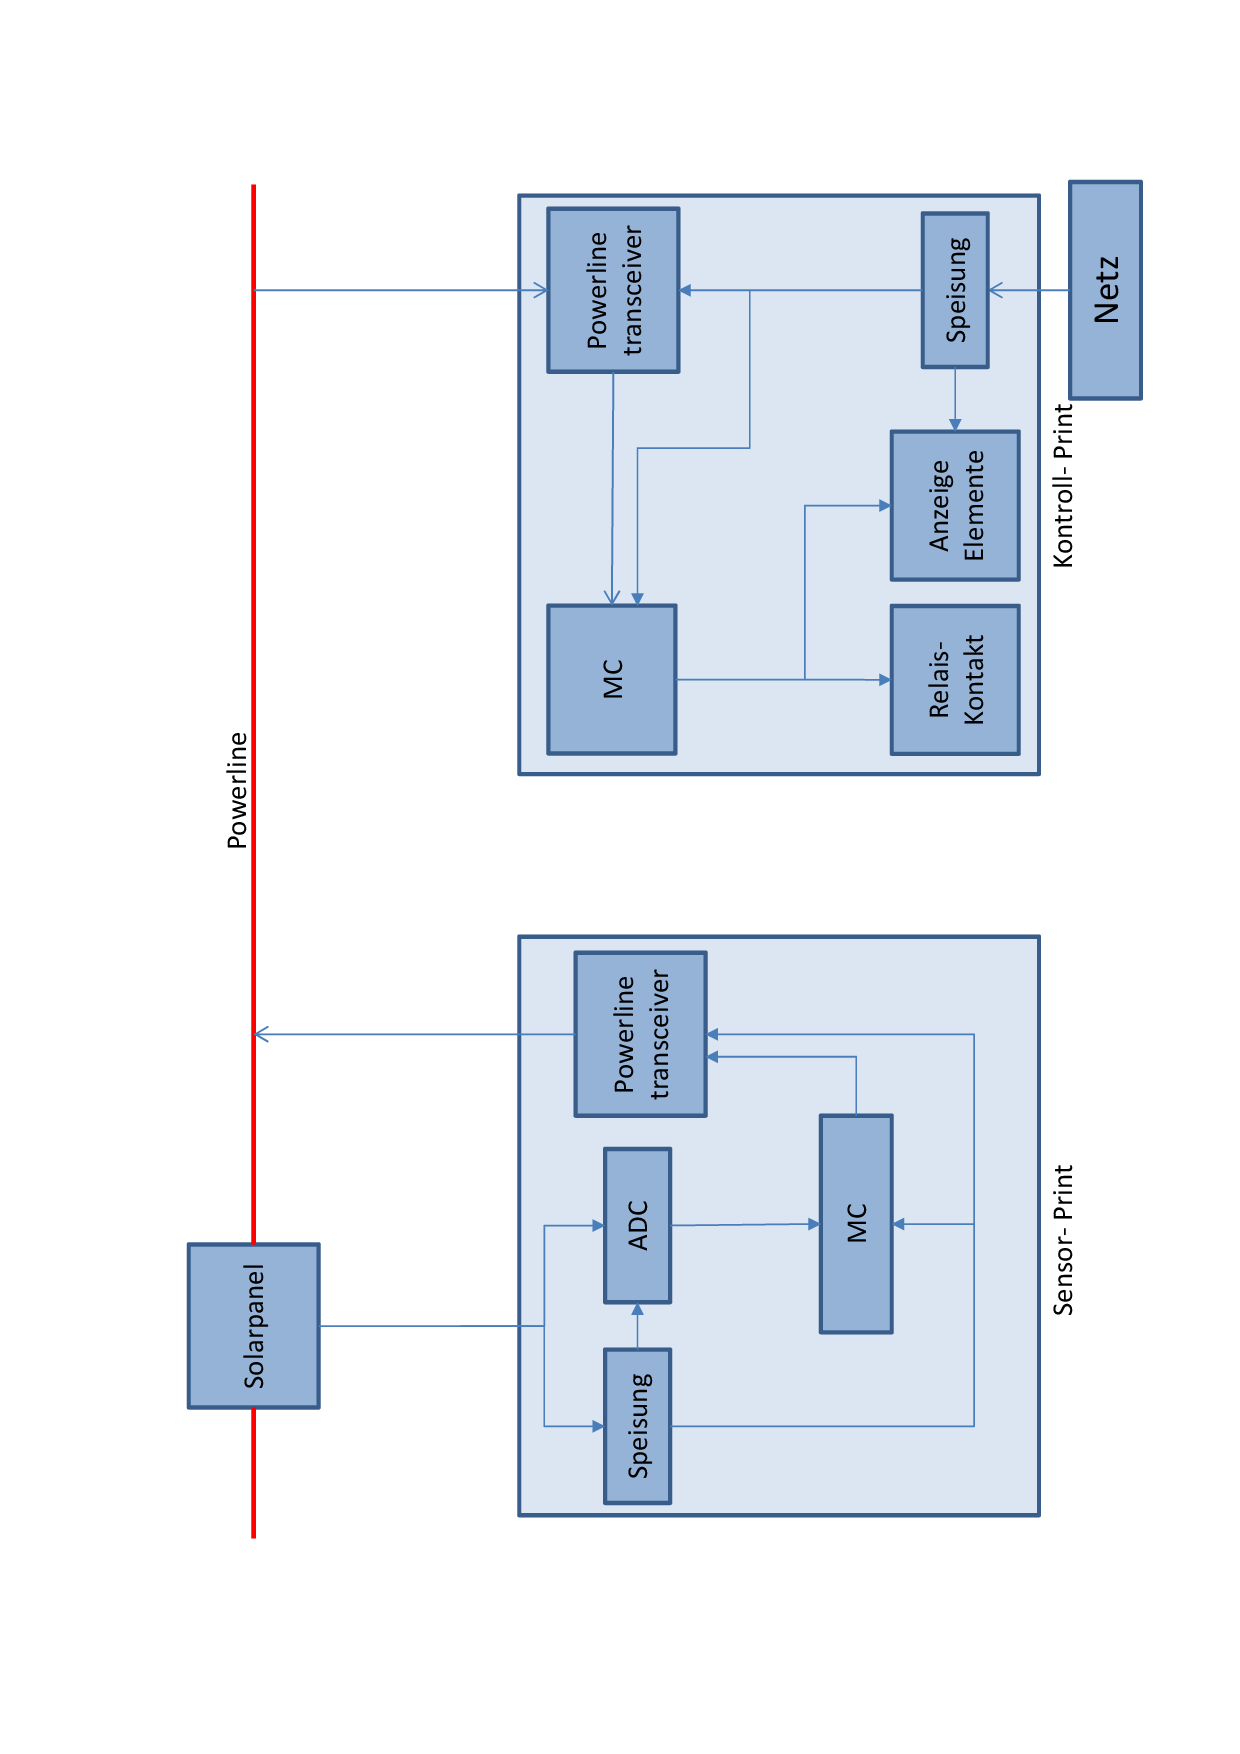
\includegraphics[angle = -90, width=1.0\textwidth]{Hardware_Konzept.png}%
\caption{Hardwarekonzept}
\label{fig::Hardwarekonzept}%
\end{figure}

\subsection{Sensorplatine}

\subsection{Kontrollplatine}
Die Kontrollplatine empfängt die modulierten Signale welche von der Sensorplatine über die Powerline übertragen werden. Diese Platine wird am Ende der Solaranlage in der Kontrollstation montiert. Dort kann der Anwender oder der Prüfer dieser Anlage herausfinden, ob defekte Solarpanels vorhanden sind.

\subsubsection{Speisung}
Die Speisung der Kontrollplatine erfolgt über das Netz. Die Netzspannung wird über ein Netzgerät auf eine definiert DC Spannung transformiert. Das Netzgerät ist noch nicht ausgewählt. Somit ist die DC Spannung noch nicht bekannt.

Die Speisung speist den Microkontroller, den Powerline transceiver und die Anzeigeelemente. Die maximale Leistung kann hier vernachlässigt werden.

\subsubsection{Powerline transceiver}
Es wird der selbe Powerline transceiver wie bei der Sensorplatine verwendet. Dieser hat die Aufgabe die Modulierten Signale über die Powerline zu empfangen und diese dann zu entmodulieren. Danach werden die verarbeiteten Signale an den Microkontroller übermittelt.

\subsubsection{Microkontroller}
Die Signale werden vom Microkontroller empfangen und abgespeichert. Wenn alle Signale abgespeichert sind, werden diese ausgewertet. Danach wird entschieden ob die einzelnen Panels funtionstüchtig oder defekt sind.

\subsubsection{Anzeige Elemente}
Als Anzeige Element wird ein Display verwendet. An diesem kann abgelesen werden, welche Panels defekt sind. Zudem sind 2 LEDs vorhanden(Grün: ok, Rot: defekt).

\subsubsection{Relais Kontakt}
Wenn die Sollspannung eines Panels nicht erreicht, steuert der Microcontroller einen Relaiskontakt an. 

%\end{document}
